\sect{Reguläre Ausdrücke}

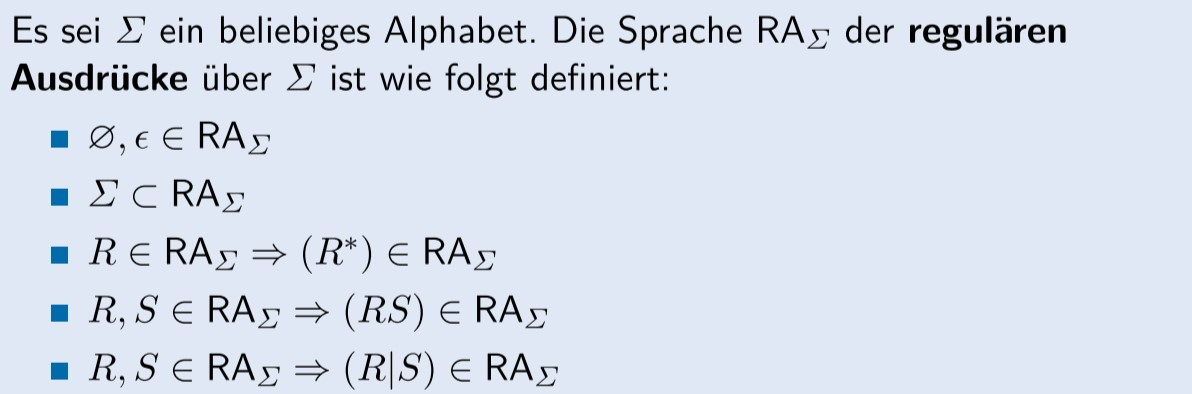
\includegraphics[scale=0.215]{regulaere-ausdruecke-definition}

Für jeden regulären Ausdruck $R \in RA_{\Sigma}$ definieren wir die Sprache $L(R)$ wie folgt:
\begin{itemize}
    \item $L(\emptyset) = \emptyset \Rightarrow$ Leere Sprache
    \item $L(\varepsilon) = {\varepsilon} \Rightarrow$ Sprache, die nur das leere Wort enthält
    \item $L(a) = \{a\}$ für $a \in \Sigma \Rightarrow$ Beschreibt die Sprache $\{a\}$
    \item $L(R^*) = L(R)^* \Rightarrow$ Kombinierte Wörter von $R$
    \item $L(R|S) = L(R) \cup L(S) \Rightarrow$ Wörter die von $R$ oder $S$ beschrieben werden
    \item $L(RS) = L(R)L(S) \Rightarrow$ Verkettungen von Wörtern ($R$ = Präfix)
\end{itemize}

Eine Sprache $A$ über dem Alphabet $\Sigma$ heisst \textbf{regulär}, falls $A = L(R)$ für einen regulären Ausdruck $R \in RA_{\Sigma}$ gilt.

\textbf{Beispiele:}
\begin{itemize}
    \item $R_1 = a^* b \Rightarrow L(R_1) = \{b, ab, aab, \dots\}$
    \item $R_2 = (aa)^* b^* aba \Rightarrow L(R_2) = \{aba, baba, aaaba, aababa, \dots\}$
    \item $R_3 = (a|ab)^* \Rightarrow L(R_3) = \{\varepsilon, a, ab, aa, abab, \dots\}$
\end{itemize}

Die Menge $RA_{\Sigma}$ ist eine Sprache über dem Alphabet $\{\emptyset, \varepsilon, *, (,), |\} \cup \Sigma$.

\textbf{Priorisierung von Operatoren:}
\begin{enumerate}
    \item $^*$ = Wiederholung
    \item Konkatenation
    \item $|$ = Auswahl
\end{enumerate}

\textbf{Beispiele:}
\begin{itemize}
    \item $(aa)^* b^* aba = (aa)^* b^* aba$
    \item $(ab)|(ba) = ab|ba$
    \item $a(b(ba))|b = abba | b$
\end{itemize}

\textbf{Erweiterte Syntax:}
\begin{multicols}{2}
    \begin{itemize}
        \item $R^+ = R(R^*)$
        \item $R? = (R|\varepsilon)$
    \end{itemize}
\end{multicols}